\documentclass[12pt,spanish]{article}
\usepackage{multicol,caption} 
\usepackage[utf8]{inputenc}  
\usepackage[spanish,english]{babel}
\usepackage{graphicx}
\usepackage{amssymb}
\usepackage{textcomp}
\usepackage{nccmath} 
\usepackage{amsmath, amsthm, amsfonts}
\usepackage{enumerate}
\usepackage{caption}
\usepackage{indentfirst} 
\usepackage{titlesec}
\usepackage{authblk}
\usepackage{hyperref}
\usepackage[none]{hyphenat}
\usepackage{apacite}
\usepackage[right=1in,left=1in,top=1in,bottom=1in,includefoot]{geometry}
\usepackage{fancyhdr}
\usepackage{lastpage}
\usepackage{enumerate}
\usepackage{wrapfig}
\usepackage{empheq}
\usepackage{mdframed}

\newcommand*\widefbox[1]{\fbox{\hspace{2em}#1\hspace{2em}}}
\renewcommand{\theenumi}{(\textit{\roman{enumi}})}
\newcommand{\myname}{Andrés F. Cerón}
\newcommand{\assignment}{Métodos Matemáticos I}
\newcommand{\duedate}{\today}
\newcommand{\Titulo}{Notas de Clase.}

\pagestyle{fancy}
\fancypagestyle{plain}
{
  \setlength{\topmargin}{-0.5in}
  \setlength{\headheight}{1.05in}
  \setlength{\headsep}{-0.0in}
  \setlength{\headwidth}{\textwidth}
  \setlength{\footskip}{2.0in}
  \fancyhead[l]{
    {\bf \assignment \hfill \myname} \\
    Departamento de Física Aplicada - Verano 2024 \hfill \today
  }
}

\pagestyle{myheadings}
\markright{\bf{Funciones analíticas.}}


\title{\Large \bf \Titulo}
\author{}
\date{}


\begin{document}

\thispagestyle{fancy}
\maketitle
\thispagestyle{plain}
\let\oldthefootnote\thefootnote

\let\thefootnote\oldthefootnote
\setlength{\headheight}{0.65in}
\setlength{\textheight}{8.60in}
\pagestyle{myheadings}

\vspace{-2cm}

\section{Números Complejos}

    \subsection{Operación Fundamentales}


        Para realizar operaciones en números complejos, se establece una independencia lineal entre los números reales e imaginarios, esto permite realizar las operaciones básicas de la siguiente forma

        \begin{enumerate}
            \item \textit{Suma}
                \begin{equation*}
                    z_1 + z_2 = (a + ib) + (c + id) = (a + c) + i (b + d)
                \end{equation*}
            \item \textit{Resta}
                \begin{equation*}
                    z_1 - z_2 = (a + ib) - (c + id) = (a - c) + i (b - d)
                \end{equation*}
            \item \textit{Multiplicación}
                \begin{equation*}
                    z_1z_2 = (a + ib)(c + id) = (ac - bd) + i(ad + bc)
                \end{equation*}
            \item \textit{División}
                \begin{equation*}
                    z_1/z_2 = (a + ib)/(c + id) = \frac{(ac + bd) + i((bc-ad))}{c^2+d^2}  
                \end{equation*}        
        \end{enumerate}

        Vale la pena recalcar que números complejos cumplen con las propiedades  \textbf{Conmutativa} y \textbf{asociativa}, tanto para la suma como para la multiplicación, adicionalmente también se cumple que el $0$ es modulo para la suma y $1$ para la multiplicación. Por último, se tiene que para todo $z_1 \neq 0$ existe un único $z$ tal que $z_1z = zz_1 = 1$, donde $z$ es llamado el inverso multiplicativo de $z_1$.
    
    \subsection{Números complejos en Forma Polar.}

        Como se expresó anteriormente, los números complejos pueden ser expresados como bases vectorial de un espacio $\mathbb{R}^2$, esto permite establecer una descripción de los complejos en términos de $r$ y $\theta$.

        \begin{wrapfigure}{l}{0.4\textwidth}
            \centering
            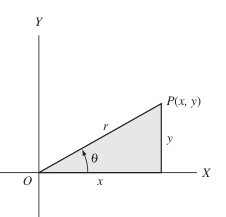
\includegraphics[width=0.4\textwidth]{imgs/ipolar.png}
            \caption{}
            \label{fig:ipl}
        \end{wrapfigure}
        Esta representación se realiza en el \textit{plano complejo} o \textit{diagrama de Argand}, donde a cada número complejo le corresponde un único punto en el plano complejo. Los ejes de este espacio son llamados eje real (para el $X$) e imaginario (para el eje $Y$).
        \vspace{0.5cm}

        Deacuerdo con Fig.\ref*{fig:ipl} para un punto $P$ se pueden establecer las siguientes relaciones

        \begin{align*}
            x = r\cos\theta &  & y = r\sin\theta
        \end{align*}

        donde $r = \sqrt{x^2 + y^2}$ es definido como el modulo de $z$, el cual se denota como $|z|$. Esto hace posible escribir entonces el número complejo en terminos de $r$ y $\theta$.

        \begin{equation*}
            z = x + iy = \cos\theta + i\sin\theta
        \end{equation*}

        Adicionalmente el ángulo $\theta$ es conocido como la fase del número complejo y tiene la forma de $\theta = \arctan(y/x)$. Usando la analogia vectorial es posible demostrar la relación existente entre los modulos de un número complejo (Ver Problema 1 - Tarea 01). Por otro lado, los modulos y fases de números complejos cumplen,
        
        \begin{gather*}
            |z_1 z_2 | = |z_1||z_2|\\
            \arg(z_1z_2) = \arg z_1 + \arg z_2
        \end{gather*}

        Donde $\arg$ es ángulo que forma el número complejo con el eje real. Otra forma bastante útil de calcular el modulo de un número complejo es mediante el complejo conjugado el cual esta definido como el cambio de signo de la parte imaginaria, es decir 

        \begin{equation*}
            z^{*} = x - iy 
        \end{equation*}

        Por tanto el modulo será 

        \begin{equation*}
            |z| = \sqrt{zz^{*}}
        \end{equation*}

    \subsection{Teorema de DeMoivre}

        Si se definen dos números complejos $z_1 = r_1(\cos\theta_1 + i\sin\theta_1)$ y $z_2 = r_2(\cos\theta_2 + i\sin\theta_2)$ tal que 

        \begin{gather*}
            z_1z_2 = r_1r_2(\cos(\theta_1 + \theta_2)+ i\sin{\theta_1 + \theta_2})\\
            z_1/z_2 = r_1r_2(\cos(\theta_1 - \theta_2)+ i\sin{\theta_1 - \theta_2})\\
        \end{gather*}

        y mediante indución matemática se generaliza este resultado se obtiene,

        \begin{gather*}
            z_1z_2\dots z_n = r_1r_2\dots r_n\left[\cos(\theta_1 + \theta_2 + \dots + \theta_n) + i\sin(\theta_1 + \theta_2 + \dots + \theta_n)\right]\\
            z^{n} = r^{n}\left(\cos\theta + i\sin\theta\right)^{n} = r^{n}(\cos{n\theta}+ i\sin{n\theta})
        \end{gather*}

        Esta última ecuación es conocida como \textit{Teorema de DeMoivre}, el cual es útil para calcular raices de números complejos. Si se quiere calcular la n-ésima raíz de un complejo

        \begin{gather*}
            z^{n} = r^{1/n}\left(\cos\theta + i\sin\theta\right)^{1/n} = r^{1/n}(\cos{(\theta/n)}+ i\sin{(\theta/n)})\\
        \end{gather*}

        Ahora como para una n-raíz deben existir $n$ valores diferentes para $z^{1/n}$

        \begin{equation*}
            z^{n} = r^{1/n}\left(\cos\theta + i\sin\theta\right)^{1/n} = r^{1/n}\left[\cos\left(\frac{\theta + 2k\pi}{n}\right) + i \sin\left(\frac{\theta + 2k\pi}{n}\right)\right]
        \end{equation*}

        Con $k = 0,1,2, \dots, n-1$ 

    \subsection{Ecuación de Euler}

        Considerando la expasión en series de \textit{Taylor} para la función exponencial.

        \begin{gather*}
            e^{i\theta} = \sum_{n = 0}^{\infty} \frac{(i\theta)^n}{n!}\\
            e^{i\theta} = \sum_{\upsilon = 0}^{\infty} \frac{(i\theta)^{2\upsilon}}{(2\upsilon)!} + \sum_{\upsilon = 0}^{\infty} \frac{(i\theta)^{2\upsilon+1}}{(2\upsilon+1)!}\\
            e^{i\theta} = \sum_{\upsilon = 0}^{\infty} (-1)^{\upsilon}\frac{\theta^{2\upsilon}}{(2\upsilon)!} + i\sum_{\upsilon = 0}^{\infty} (-1)^{\upsilon}\frac{\theta^{2\upsilon+1}}{(2\upsilon+1)!}\\
        \end{gather*}

        Si se tiene encuenta la expasión en series de Taylor para las funciones seno y coseno

        \begin{align*}
            \cos\theta = \sum_{\upsilon = 0}^{\infty} (-1)^{\upsilon}\frac{\theta^{2\upsilon}}{(2\upsilon)!} && \sin\theta = \sum_{\upsilon = 0}^{\infty} (-1)^{\upsilon}\frac{\theta^{2\upsilon+1}}{(2\upsilon+1)!}
        \end{align*}

        remplazando se obtiene la \textit{Ecuación de Euler} 

        \begin{equation*}
            e^{i\theta} = \cos\theta + i\sin\theta
        \end{equation*}

        Esta ecuación permite establecer una relacion con el teorema de DeMoivre, de tal manera que es posible escribir,

        \begin{gather*}
            z^{n} = r^{n}(e^{in\theta}) = r^{n}(\cos{n\theta}+ i\sin{n\theta})\\
            e^{in\theta} = \cos{n\theta}+ i\sin{n\theta}\\
        \end{gather*}


        \subsubsection{Algunas propiedades utiles}
\section{Funciones Complejas}
    
Todas las funciones elementales de variables reales pueden ser extendidas al plano complejo, con solo cambiar la variable real $x$ por una variable compleja $z$.

\subsection[short]{Condiciones de Cauchy-Riemann}

    Partiendo de una función de variable compleja estable $f(z)$, se define su derivada tal cual como una función real.

    \begin{equation*}
        \lim_{\delta z \rightarrow 0} \frac{f(z + \delta z) - f(\delta z)}{z + \delta z - z} = \frac{\delta f}{\delta z} = \frac{df}{dz}
    \end{equation*}
    siempre que el limite sea \textbf{independiente} a la aproximación particular al punto $z$, es decir, que para que el límite exista las aproximaciones con $\delta y = 0$  y $delta x = 0$  deben ser iguales. Eso es debido a que en una función compleja hay dos formas en las que podemos aproximarnos a un limites (tal como lo muestra la Fig.\ref*{fig:ich})

    \begin{figure}[h]
        \centering
        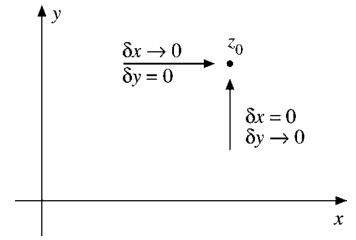
\includegraphics[width=0.4\textwidth]{imgs/ich.png}
        \caption{}
        \label{fig:ich}
    \end{figure}
    Considerando incrementos en $x$ y en $y$ entonces, 

    \begin{gather*}
        \delta z = \delta x + i\delta y\\
    \end{gather*}

    Ahora, teniendo en cuenta que $f  = u(x,y) + iv(x,y)$ entonces 
    \begin{gather*}
        \delta f = \delta u + i \delta v
    \end{gather*}

    por tanto,

    \begin{equation*}
        \frac{\delta f}{\delta z} = \frac{\delta u + i\delta v}{\delta x + i\delta y}
    \end{equation*}
    
    Realizando la aproximación al limite cuando $\delta y = 0$ y $\delta x \rightarrow 0$

    \begin{equation*}
        \lim_{\delta z \rightarrow 0}  \frac{\delta f}{\delta z} = \lim_{\delta x \rightarrow 0} \left(\frac{\delta u}{\delta x}+ i\frac{ \delta v}{\delta x}\right) = \frac{\partial u}{\partial x} + i \frac{\partial v}{\partial x}
    \end{equation*}
    para cuando $\delta x = 0$ y $\delta y \rightarrow 0$ 
    \begin{equation*}
        \lim_{\delta z \rightarrow 0}  \frac{\delta f}{\delta z} = \lim_{\delta y \rightarrow 0} \left(\frac{\delta u}{i\delta y}+ \frac{ \delta v}{\delta y}\right) = - i\frac{\partial u}{\partial y} + \frac{\partial v}{\partial y}
    \end{equation*}
    entonces para que el limite exista se debe cumplir

    \begin{gather*}
        \lim_{\delta x \rightarrow 0} \left(\frac{\delta u}{\delta x}+ i\frac{ \delta v}{\delta x}\right) = \lim_{\delta y \rightarrow 0} \left(\frac{\delta u}{i\delta y}+ \frac{ \delta v}{\delta y}\right)\\
        \frac{\partial u}{\partial x} + i \frac{\partial v}{\partial x} = - i\frac{\partial u}{\partial y} + \frac{\partial v}{\partial y}
    \end{gather*}
    ahora como $\Im$ y $\Re$ son linealmente independientes entonces 

    \begin{align*}
        \frac{\partial u}{\partial x} =  \frac{\partial v}{\partial y} && \frac{\partial v}{\partial x} = - \frac{\partial u}{\partial y}
    \end{align*}
    estas son las \textit{condiciones de Cauchy-Riemann} y se tienen que cumplir para que la derivada de una función compleja exista, ahora cambiando un poco la notación se establece que

    \begin{gather*}
        \frac{\partial u}{\partial x} =  \frac{\partial v}{\partial y}  \longrightarrow  U_x = V_y\\
        \frac{\partial v}{\partial x} =  -\frac{\partial u}{\partial y}  \longrightarrow  V_x = -U_y\\
    \end{gather*}

    Para una función de variable compleja que cumpla con las condiciones de Cauchy-Riemann y las derivadas parciales sobre $u(x,y)$ y $v(x,y)$ son continuas entonces se puede escribir

    \begin{gather*}
        \frac{\delta f}{\delta z} = \frac{(U_x + iV_x)\delta x + (U_y + iV_y)\delta y}{\delta x + i\delta y}
    \end{gather*}

    




\section{Integrales}

\subsection{Integrales definidas de funciones de variable real}

Considere el caso de una función compleja pero que dependa de una variable real $t$, esto implica entonces 

\begin{gather}
    w(t) = u(t) + iv(t)
\end{gather}
donde $u$ y $v$ son funciones de \textit{valor real} de la variable $t$. Esto permite entonces definir su derivada como 

\begin{gather}
    w^{\prime}(t) = u^{\prime}(t) + iv^{\prime}(t)
\end{gather}
esto permite concluir que $w(t)$ es una función de \textit{valor complejo} que esta compuesta por dos funciones de valor real. Por tanto una integración sobre una función compleja esta definida como la integración de dos funciones de valor real.

\begin{gather}
    \int_{a}^{b}w(t)dt = \int_{a}^{b}u(t)dt + i\int_{a}^{b}v(t)dt
\end{gather}
esto implica que para que la integral exista, entonces las funciones $u$ y $v$ deben ser continuas a trozos en el intervalo $a \leq t \leq b$. Debido a que la integración de una función compleja de variable real desemboca en dos integrales de funciones reales entonces las propiedades estudiadas sobre funciones reales se cumplirán de la misma forma. Es entonces que debido al teorema fundamental del cálculo se cumple 

\begin{gather}
    \int_{a}^{b}w(t)dt =  \left.U(t)\right|_a^{b} + iV(t)|_a^{b} = [U(b) + iV(b)] - [U(a) + iV(a)]
\end{gather}
Pese a que muchas de las reglas del calculo integral se cumplen para funciones complejas de variable real, existen excepciones como lo puede ser el caso del teorema de valor medio. 

\subsection{Contornos}

Las integrales de funciones complejas con \textbf{variable compleja} se definen sobre curvas en el plano complejo, y no sólo en intervalos de la recta real.\newline \\
Un conjunto de puntos $z = (x, y)$ en el plano complejo se dice que es un arco si

\begin{align*}
    x = x(t), && y = y(t) && (a \leq t \leq b)
\end{align*}
donde $x(t)$ y $y(t)$ son funciones continuas del parámetro real $t$. Esta definición establece un mapeo continuo del intervalo $a \leq t \leq b$ dentro del plano $xy$ y los puntos de la imagen se ordenan según valores crecientes de $t$. Es entonces conveniente los puntos de $C$ mediante la ecuación 

\begin{align}
    \label{eq:s3.2-1}z = z(t) && \text{donde}&& z(t) = x(t) + iy(t) 
\end{align}
estos corresponden a los puntos del plano complejo sobre una curva que corresponden a los valores reales que se encuentran dentro del intervalo $a \leq t \leq b$. Si la curva no se intercepta así misma entonces se dice que es un arco simple, pero si esta curva se intercepta solo en el punto $z(a) = z(b)$, entonces se dice que es una curva cerrada simple.\newline \\
La representación paramétrica utilizada para cualquier arco C no es única, de hecho, es posible cambiar el intervalo sobre el que se extiende el parámetro a cualquier otro intervalo.

\begin{gather}
    t = \phi(\tau) \;\;\;\; (\alpha \leq \tau \leq \beta)
\end{gather}
donde $\phi$ es función de valor real mapeada en un intervalo  $\alpha \leq \tau \leq \beta$ dentro del intervalo $a \leq t \leq b$. Donde $\phi$ y su derivada deben ser continuas, esto permite realizar una transformación sobre la ecuación (\ref*{eq:s3.2-1})

\begin{align}
    z = z[\phi(\tau)] && (\alpha \leq \tau \leq \beta)
\end{align}
Suponga ahora las componentes $x^{\prime}(t)$ y $y^{\prime}(t)$ de la derivada de la función $z(t)$, esto permite definir una función de valor real llamada arco diferenciable

\begin{gather*}
    |z^{\prime}(t)| = \sqrt{[x^{\prime}(t)]^2 + [y^{\prime}(t)]^2}
\end{gather*}
recordando que la definición de longitud de arco en calculo integral estaba dada por

\begin{gather*}
    L = \int_{a}^{b}|z^{\prime}(t)|dt 
\end{gather*}
debido a que la longitud de arco debe permanecer invariante ante ciertas transformaciones, entonces es posible re definir esta ecuación de la siguiente forma

\begin{gather*}
    L = \int_{a}^{b}|z^{\prime}[\phi(\tau)]|\phi^{\prime}(\tau)d\tau 
\end{gather*}
esto permite demostrar que la longitud de $C$ será la misma ante parametrizaciones de la curva.\newline\\ 
Los puntos de cualquier curva simple cerrada o contorno simple cerrado $C$ son puntos límite de dos dominios distintos, uno de los cuales es el interior de $C$ y está acotado, el otro que es el exterior de $C$ y no está acotado.

\subsection{Integrales de contorno}

Las integrales de funciones complejas $f$ de variable compleja $z$ están definidas en términos de los valores $f(z)$ a lo largo de un contorno dado $C$, que se prolonga de un punto $z = z_1$ a otro $z = z_2$ contenidos en el plano complejo, es decir, una integral de linea; y su valor depende en general tanto del contorno $C$ como de la función $f$. Se definirá la integración de estas funciones en términos de integración de funciones de valor real, para tal propósito suponga la función 

\begin{gather*}
    z = z(t) \;\;\;\;\;\; (a \leq t \leq b)
\end{gather*}
que representa el contorno $C$, el cual va del punto $z_1 = z(a)$ a $z_2 = z(b)$. También se asume que $f[z(t)]$ es una función continua a trozos dentro del intervalo y nos referimos entonces a la función $f(z)$ continua dentro del contorno $C$. Esto permite definir la integral de linea o \textbf{integral de contorno} de $f$ a lo largo de $C$ en términos del parámetro $t$ 

\begin{gather*}
    \int_C f(z)dz = \int_{a}^{b}f[z(t)]z^{\prime}(t)dt
\end{gather*}
El resultado de esta integral resulta ser invariante ante parametrizaciones como se concluyó anteriormente. Este resultado permite entonces establecer las propiedades de esta integración 

\begin{gather*}
    \int_C z_0f(z)dz = z_0\int_C f(z)dz\\
    \int_C [f(z) + g(z)]dz = \int_C f(z)dz + \int_C  g(z)dz\\
    \int_{-C} f(z)dz = -\int_C f(z)dz\\
    \int_{a}^{b}f[z(t)]z^{\prime}(t)dt = \int_{a}^{c}f[z(t)]z^{\prime}(t)dt + \int_{c}^{b}f[z(t)]z^{\prime}(t)dt \\
    \int_{C}f(z)dz = \int_{C_1}f(z)dz + \int_{C_2}f(z)dz
\end{gather*}

\subsection{Antiderivadas}

Aunque el valor de una integral de contorno de una función $f(z)$ desde un punto fijo $z_1$ a otro punto fijo $z_2$ depende, en general, del camino que se recorra, hay ciertas funciones cuyas integrales tienen valores independientes del recorrido.

\begin{mdframed}
    \textbf{Teorema:}\\
Suponga que una función $f(z)$ es continua en un dominio $D$. Si una de las siguientes afirmaciones es correcta entonces las otras también lo serán.

\begin{enumerate}
    \item $f(z)$ tiene una antiderivada $F(z)$ en todo $D$
    \item Las integrales de $f(z)$ a lo largo de los contornos situados enteramente en $D$ y que se extienden desde cualquier punto fijo $z_1$ a cualquier punto fijo $z_2$ tienen todas el mismo valor.
    \item Las integrales de $f(z)$ alrededor de contornos cerrados situados enteramente en D tienen todas valor cero.
\end{enumerate}
\end{mdframed}
Hay que resaltar que el teorema no afirma que alguna de estas afirmaciones sea cierta para una función $f(z)$ dada, sólo dice que todas ellas son verdaderas o que ninguna de ellas lo es.

\subsection{Teorema de Cauchy-Goursat}

Suponga un contorno simple cerrado $C$ denotado por la función $z = z(t)$ en el intervalo  $a \leq t \leq b$, adicionalmente considere que esta descrito en dirección positiva. Ahora suponga una función $f$ que es analítica para todo punto dentro de $C$, mediante una parametrización se establece que la integral de esta función sobre $C$ será 

\begin{gather}
    \int_C f(z)dz = \int_{a}^{b}f[z(t)]z^{\prime}(t)dt
\end{gather}
donde 

\begin{align*}
    f(z) = u(x,t) + i(x,y) && z(t) = x(t) + iy(t)
\end{align*}
esto implica entonces la parametrización

\begin{gather*}
    f[z(t)] = u[x(t), y(t)] + iv[x(t),y(t)]
\end{gather*}
remplazando

\begin{gather*}
    \int_C f(z)dz = \int_{a}^{b} \left( u[x(t), y(t)] + iv[x(t),y(t)]\right)\left(x^{\prime}(t) + iy^{\prime}(t)\right)dt\\
    \int_C f(z)dz = \int_{a}^{b} \left( ux^{\prime} - vy^{\prime}\right)dt     + i\int_{a}^{b}\left(vx^{\prime} + uy^{\prime}\right)dt
\end{gather*}
en términos de integrales de línea de funciones de valor real de dos variables reales, recordando que $x^{\prime} = dx/dt$ y $y^{\prime} = dy/dt$ 

\begin{gather}
    \int_C f(z)dz = \int_{C} \left( u dx - vdy\right) + i\int_{C}\left(v dx + udy\right)
\end{gather}
esta expresión es valida para cualquier contorno $C$, siempre y cuando $f[z(t)]$ sea continua a trozos dentro del contorno. \newline \\
Recordando que el teorema de green establece que para dos funciones $P(x,y)$ y $Q(x,y)$, que junto con sus derivadas parciales de primer orden, son continuas dentro de una región $R$ que contiene todos los puntos interiores y sobre el contorno simple cerrado $C$, se cumple 

\begin{gather}
    \int_C Pdx + Qdy  = \int\int_R (Q_x - P_y)dA
\end{gather}
como $f$ será continua en $R$, debido a que es analítica para todo $C$. Entonces las funciones $u$ y $v$ también serán continuas en $R$, esto implica entonces 

\begin{gather*}
    \int_C f(z)dz = \int\int_R (-v_x - u_y)dA  + i\int\int_R (u_x - v_y)dA
\end{gather*}
debido a que $f$ es analítica, entonces debe cumplir con las condiciones de Cauchy-Riemann $u_x = v_y, -v_x = u_y$, remplazando 

\begin{gather}
    \int_C f(z)dz = \int\int_R (u_y - u_y)dA  + i\int\int_R (v_y - v_y)dA = 0
\end{gather}
Una vez establecido que el valor de esta integral es cero,
la orientación de $C$ es irrelevante, esto implica

\begin{gather*}
    \int_C f(z)dz = - \int_{-C} f(z)dz  = 0
\end{gather*}
Goursat fue el primero en demostrar que la condición de continuidad sobre $f^{\prime}$ puede ser omitida.

\begin{mdframed}
    \textbf{Teorema:}\\
Si una función $f$ es analítica en todos los puntos interiores y en un contorno cerrado simple $C$, entonces

\begin{gather}
    \int_C f(z)dz = 0
\end{gather}
\end{mdframed}

\subsection{Dominios Simplemente Conexos}

Un dominio simplemente conexo $D$ es un dominio tal que cada contorno cerrado simple dentro de él, solo encierre puntos de $D$, es decir, que contornos cerrados dentro del dominio solo pueden encerrar puntos pertenecientes a $D$. 

\begin{mdframed}
    \textbf{Teorema:}\\
Si una función $f$ es analítica en un dominio $D$ simplemente conexo, entonces
\begin{gather}
    \int_C f(z)dz = 0
\end{gather}
para todo contorno cerrado $C$ situado en $D$.
\end{mdframed}
La demostración es fácil si $C$ es un contorno cerrado simple o si es un contorno cerrado que se interseca a sí mismo un número finito de veces. Porque si $C$ es simple y está en $D$, la función f es analítica en cada punto interior a y sobre $C$; y el teorema de Cauchy asegura que se cumple la ecuación. Para el caso en que $C$ se intersecta un número finito de veces forma un número finito de contornos cerrados simples, donde el teorema de Cauchy se cumple para cada uno.

\begin{gather*}
    \int_C f(z)dz  = \sum_{k=1}^{N} \int_{C_k}f(z)dz = 0
\end{gather*}
\textbf{Ejemplo:}\\
Si $C$ denota un contorno cerrado contenido en un disco abierto $|z| <2$, entonces 

\begin{gather*}
    \int_C \frac{ze^z}{(z^2 + 9)^5} = 0
\end{gather*}
esto se cumple debido a que las singularidades de esta función ($z \pm 3i$) se encuentran fuera del disco.
\begin{mdframed}
    \textbf{Corolario:}\\
    Una función $f$ que es analítica en todo un dominio simplemente conexo $D$ debe tener una antiderivada en cualquier parte de $D$. 
\end{mdframed}

\subsection{Dominios Multiconexos}
Se dice que un dominio que no es simplemente conexo (Sec. 48) es conexo múltiple.
\begin{mdframed}
    \textbf{Teorema:}\\
    Suponga que
    \begin{enumerate}
        \item  $C$ es contorno cerrado simple, descrito en la dirección contraria a las manecillas del reloj.
        \item $C_k$ son contornos cerrados simples interiores a $C$, todos descritos en dirección a las manecillas del reloj, que son disjuntos y cuyos interiores no tengan puntos en común
    \end{enumerate}
    Si una función $f$ es analítica en todos estos contornos y en todo el dominio multiconexo, es decir, en los puntos interiores a $C$ y exteriores a cada $C_k$, entonces
    \begin{gather*}
        \int_{C} f(z)dz + \sum_{k=1}^{n}\int_{C_k}f(z)dz = 0
    \end{gather*}
\end{mdframed}
Obsérvese que en esta ecuación, la dirección de cada trayectoria de integración es tal que el dominio de multiconexo se encuentra a la izquierda de dicha trayectoria.

\begin{mdframed}
    \textbf{Corolario:}\\
    Sean $C_1$ y $C_2$ contornos cerrados simples orientados positivamente, donde $C_1$ es interior a $C_2$. Si una función $f$ es analítica para todos los puntos en la región que esta encerrada entre ambos contornos, entonces 
    \begin{gather*}
        \int_{C_2} f(z)dz = \int_{C_2}f(z)dz
     \end{gather*}
\end{mdframed}
Este corolario es conocido como el principio de deformación de caminos, ya que, dice que si $C_1$ se deforma continuamente en $C_2$, pasando siempre por los puntos en donde $f$ es analítica, entonces el valor de la integral de $f$ sobre $C_1$ nunca cambia.\newline
\textbf{Ejemplo:}\\
Demostrar que 
\begin{gather*}
    \int_C \frac{dz}{z} = 2\pi i
\end{gather*}
Para ello, se construye una circunferencia de orientación positiva $C_0$ con centro en el origen y radio tan pequeño que $C_0$ se encuentra completamente dentro de $C$.

\begin{gather*}
    \int_{C_0} \frac{dz}{z} = \int_{-\pi}^{+\pi}\frac{iRe^{i\theta}}{Re^{i\theta}}d\theta = i\int_{-\pi}^{+\pi}d\theta = 2\pi i
\end{gather*}
Y como $1/z$ es analítica en todas partes menos en $z=0$, entonces mediante el principio de deformación de caminos.

\begin{gather*}
    \int_C \frac{dz}{z} = \int_{C_0} \frac{dz}{z} = 2\pi i
\end{gather*}

\subsection{Integral de Cauchy}
\begin{mdframed}
    \textbf{Teorema:}\\
    Suponga una función $f$ que es analítica para todo el interior de un contorno cerrado simple $C$, descrito en sentido positivo. Si $z_0$ es un punto interior a $C$, entonces
    \begin{gather*}
        f(z_0) = \frac{1}{2\pi i }\int_C \frac{f(z)dz}{z-z_0}
    \end{gather*}
\end{mdframed}
esta expresión es conocida como la integral de Cauchy. Dice que si una función $f$ es analítica dentro y sobre un contorno cerrado simple $C$, entonces los valores de $f$  en el interior de $C$ están completamente determinas por los valores de $f$ sobre $C$.

\begin{gather*}
    \int_C \frac{f(z)dz}{z-z_0} = 2\pi if(z_0)
\end{gather*}
\textbf{Ejemplo:}\\
Sea $C$ un circulo de radio $|z| = 2$, orientado positivamente. Considere también la siguiente función

\begin{gather*}
    f(z) = \frac{z}{9 - z^2}
\end{gather*}
como esta función es analítica dentro y sobre $C$, debido a que $z_0 = -i$ está dentro de $C$, entonces

\begin{gather*}
    \int_C \frac{zdz}{(9-z^2)(z+i)} = \int_C \frac{z/(9 - z^2)}{z - (-i)}dz = 2\pi if(-i) = 2\pi i \frac{-i}{10} = \frac{\pi}{5}
\end{gather*}

\subsection{Extensión de la integral de Cauchy}
La integración de Cauchy puede ser extendida para proporcionar una representación integral de las derivadas de $f$ evaluadas en $z_0$. Para tal objetivo se supondrá una función $f$ que es analítica sobre y en todo el interior de un contorno cerrado simple $C$, descrito en sentido positivo. Es decir, se cumplirá el teorema de la integral de Cauchy

\begin{gather}
    f(z) = \frac{1}{2\pi i}\int_C \frac{f(s)ds}{s-z}
\end{gather}
donde $z$ es un punto interior a $C$ y $s$ son todos los puntos contenidos en $C$. Derivando respecto a $z$ ambos lados de la igualdad,

\begin{gather*}
    f^{\prime}(z) = \frac{1}{2\pi i}\int_C \frac{f(s)ds}{(s-z)^2}
\end{gather*}
esta expresión se puede generalizar (demostrando la existencia de las integrales)

\begin{gather*}
    f^{(n)}(z) = \frac{n!}{2\pi i}\int_C \frac{f(s)ds}{(s-z)^{n+1}}
\end{gather*}
expresando esta generalidad de la siguiente forma

\begin{gather}
    \int_C \frac{f(z)}{(z - z_0)^{n+1}} = \frac{2\pi i}{n!}f^{(n)}(z_0)
\end{gather}
estas expresiones pueden ser útiles para evaluar ciertas integrales cuando $f$ es analítica dentro y sobre un contorno cerrado simple $C$, tomado en sentido positivo, y $z_0$ es cualquier punto interior a $C$.



\end{document}
